%this is template for my % Template for INT1414 reports
%% by Thanh Le
%% based on LaTeX work of Robin Turner.
%% Adapted from the IEEE peer review template


\documentclass[conference]{IEEEtran}
\IEEEoverridecommandlockouts
\usepackage{cite} % Tidies up citation numbers.
\usepackage{url} % Provides better formatting of URLs.
\usepackage{booktabs} % Allows the use of \toprule, \midrule and \bottomrule in tables for horizontal lines
\usepackage{graphicx}

\usepackage{listings}
\usepackage{xcolor}

% Define custom colors
\definecolor{codegreen}{rgb}{0,0.6,0}
\definecolor{codegray}{rgb}{0.5,0.5,0.5}
\definecolor{codepurple}{rgb}{0.58,0,0.82}
\definecolor{backcolour}{rgb}{0.95,0.95,0.92}

% Configure the global style for listings
\lstset{
    backgroundcolor=\color{backcolour},   
    commentstyle=\color{codegreen},
    keywordstyle=\color{magenta},
    numberstyle=\tiny\color{codegray},
    stringstyle=\color{codepurple},
    basicstyle=\footnotesize\ttfamily,
    breakatwhitespace=false,         
    breaklines=true,                 
    captionpos=b,                    
    keepspaces=true,                 
    numbers=left,                    
    numbersep=5pt,                  
    showspaces=false,                
    showstringspaces=false,
    showtabs=false,                  
    tabsize=2,
    frame=single,
    rulecolor=\color{black},
    title=\lstname
}
\hyphenation{op-tical net-works semi-conduc-tor} 

\usepackage{amsmath,amssymb,amsfonts}
\usepackage{algorithmic}
\usepackage{textcomp}
\usepackage{xcolor}
\def\BibTeX{{\rm B\kern-.05em{\sc i\kern-.025em b}\kern-.08em
    T\kern-.1667em\lower.7ex\hbox{E}\kern-.125emX}}


\begin{document}
\title{Deployment and Analysis of a Distributed PostgreSQL Database System Using the Pagila Dataset}

\author{\IEEEauthorblockN{Huynh Minh Thinh}
\IEEEauthorblockA{\textit{Department of Information Technology 2} \\
\textit{Posts and Telecommunications Institute of Technology at HCM city}\\
Ho Chi Minh City, Vietnam \\
D22CQCN01-N \\
n22dccn082@student.ptithcm.edu.vn}}
\date{09/06/25}

\maketitle

\begin{abstract}
For this project, I tackled the common challenge of building a database that can handle both heavy user traffic and unexpected server failures. I constructed a four-node PostgreSQL 17 cluster, using one primary server to handle all data changes and three hot-standby replicas to manage read requests. To make the system resilient, I used native streaming replication enhanced with dedicated replication slots, which guarantees that a standby server can always reconnect without losing its place in the data stream. I built this system on a KVM virtualized environment and used the Pagila sample database to simulate a realistic workload for a physical DVD rental store. My analysis confirmed that this architecture can effectively distribute read queries to prevent performance bottlenecks and can maintain read-only service even when the primary server fails. Ultimately, this project demonstrates that this replication model is a strong and practical foundation for building scalable and reliable web applications, with clear next steps like automated failover being the path toward a production-ready system.


\end{abstract}





\section{Introduction}

In today's digital world, a single database can struggle to keep up with the demands of a successful application. As more users connect and more data is collected, a traditional database can become a bottleneck, slowing everything down or even crashing entirely. Worse, if that single server fails, everything can be lost. A popular and effective solution to this problem is to move away from a single database and instead use a "distributed" system that spreads the work across multiple computers.

This project puts that solution into practice. I set out to build and analyze a small network—or cluster—of four PostgreSQL databases working together. Using PostgreSQL's own streaming replication feature, I configured one main "primary" server and three "hot-standby" replicas. This kind of setup is an industry standard for making sure a system stays online (high availability) and can handle many users reading data at once (read scalability). To test the cluster with realistic information, I loaded it with the Pagila sample dataset, which is designed to look like the database for a video rental store.

This report will walk you through the entire project. It starts by explaining the core problem of scaling a database and how replication helps solve it. I'll then cover the step-by-step process of setting up the virtual machines, configuring the main server and its replicas, and loading the Pagila data. After that, I will analyze how well this setup would support a busy web application, and I'll finish by summarizing what I learned and suggesting ideas for the future.
\section{Problem Definition}
Any successful website eventually hits two walls. The first is the "too popular" problem: so many people are using the site at once that it slows to a crawl. The second is the "everything is broken" problem: a single server fails, and the entire site goes offline.

For an online DVD rental service, the "too popular" issue comes from having thousands of users Browse the catalog simultaneously. Most of what they do—searching for films, reading descriptions, checking actor pages—are read operations. These requests quickly overwhelm a single database server, leading to frustratingly slow load times for everyone.

The "everything is broken" problem is even more severe. If our one and only database server crashes, there is no backup. The entire service becomes unavailable, losing customers and revenue. This project's goal is to build a database system that solves both these problems: one that can handle a massive read workload without slowing down, and one that can survive a server failure without shutting down completely.

\section{Proposed Solutions}

With the main goals of speed and reliability in mind for a future large-scale site, I had to make a big decision right at the start: how should the data be organized across multiple servers? It really boiled down to two main philosophies: splitting the data up, or making copies of it.


\subsection{The "Divide and Conquer" Method: Sharding}
The first philosophy, sharding, is like deciding to replace one massive, central filing cabinet with several smaller ones. You'd organize them by a clear rule—for example, putting all customer files for names A-M in the first cabinet, and N-Z in the second.

The big advantage here is that you can have multiple people filing new documents at the same time, which is fantastic for handling a huge volume of new data (writes). The real challenge, though, is the new complexity. Your application now has to act like a smart receptionist, knowing exactly which cabinet to send someone to for a specific file. Any task that needs information from both cabinets, like a company-wide report, becomes a real puzzle to solve.

\subsection{The "Make a Copy" Method: Replication (My Chosen Solution)}
The other philosophy, and the one I chose for this project, is replication. Instead of splitting up the filing cabinet, I decided to keep the original as the one "master" source of truth, and then create several perfect duplicates.

The system operates on a simple rule: any new information (a write) must go to the master cabinet first. Once it's there, an identical copy of the update is immediately sent out to all the duplicate cabinets. The payoff for this is huge. When a hundred people need to look something up (a read), they can be sent to any of the available copies. This keeps the line at the master cabinet short, leaving it free to handle new, incoming information.


\section{Criteria for Assessing Solutions} \label{sec:criteria}
I chose replication over sharding because of three important factors that were directly related to the project's goals:

\begin{itemize}
    \item \textbf{Alignment with Workload:} The target application, which is a DVD rental service, is mostly read-heavy. Replication makes read-only copies to deal with this directly, while sharding is mostly used for workloads that need a lot of writing.

    \item \textbf{Path to High Availability:} Replication makes it easy to set up high availability because any standby server is a full copy of the data that can be used as a primary.
    \item \textbf{Implementation Simplicity:} Native streaming replication is a core feature of PostgreSQL that is easy to use and well-documented. It doesn't need complicated changes to the application-level logic, which makes it much easier to set up correctly than a sharded architecture.
\end{itemize}

Replication was the best and most practical solution for this project based on these factors. 


\section{Implementation Methodology}

\subsection{System Environment and Network Configuration}

I built my four-node cluster using a mix of my main computer and some virtual ones. My physical machine was the primary server, and I ran the three standby servers as virtual machines (VMs) right on that same computer. To do this, I used KVM/QEMU for the virtualization part, managed with the `virt-manager` program.

To get all these servers talking to each other, I put them all on their own private network (`192.168.122.0/24`). This kept the important database traffic separate from everything else. A crucial step was giving each server a static IP address, which is essential for stable replication. The overall architecture is illustrated in Figure \ref{fig:architecture}, and the specific node details are listed in Table \ref{tab:node_config}.

\begin{figure}[!h]
    \centering
    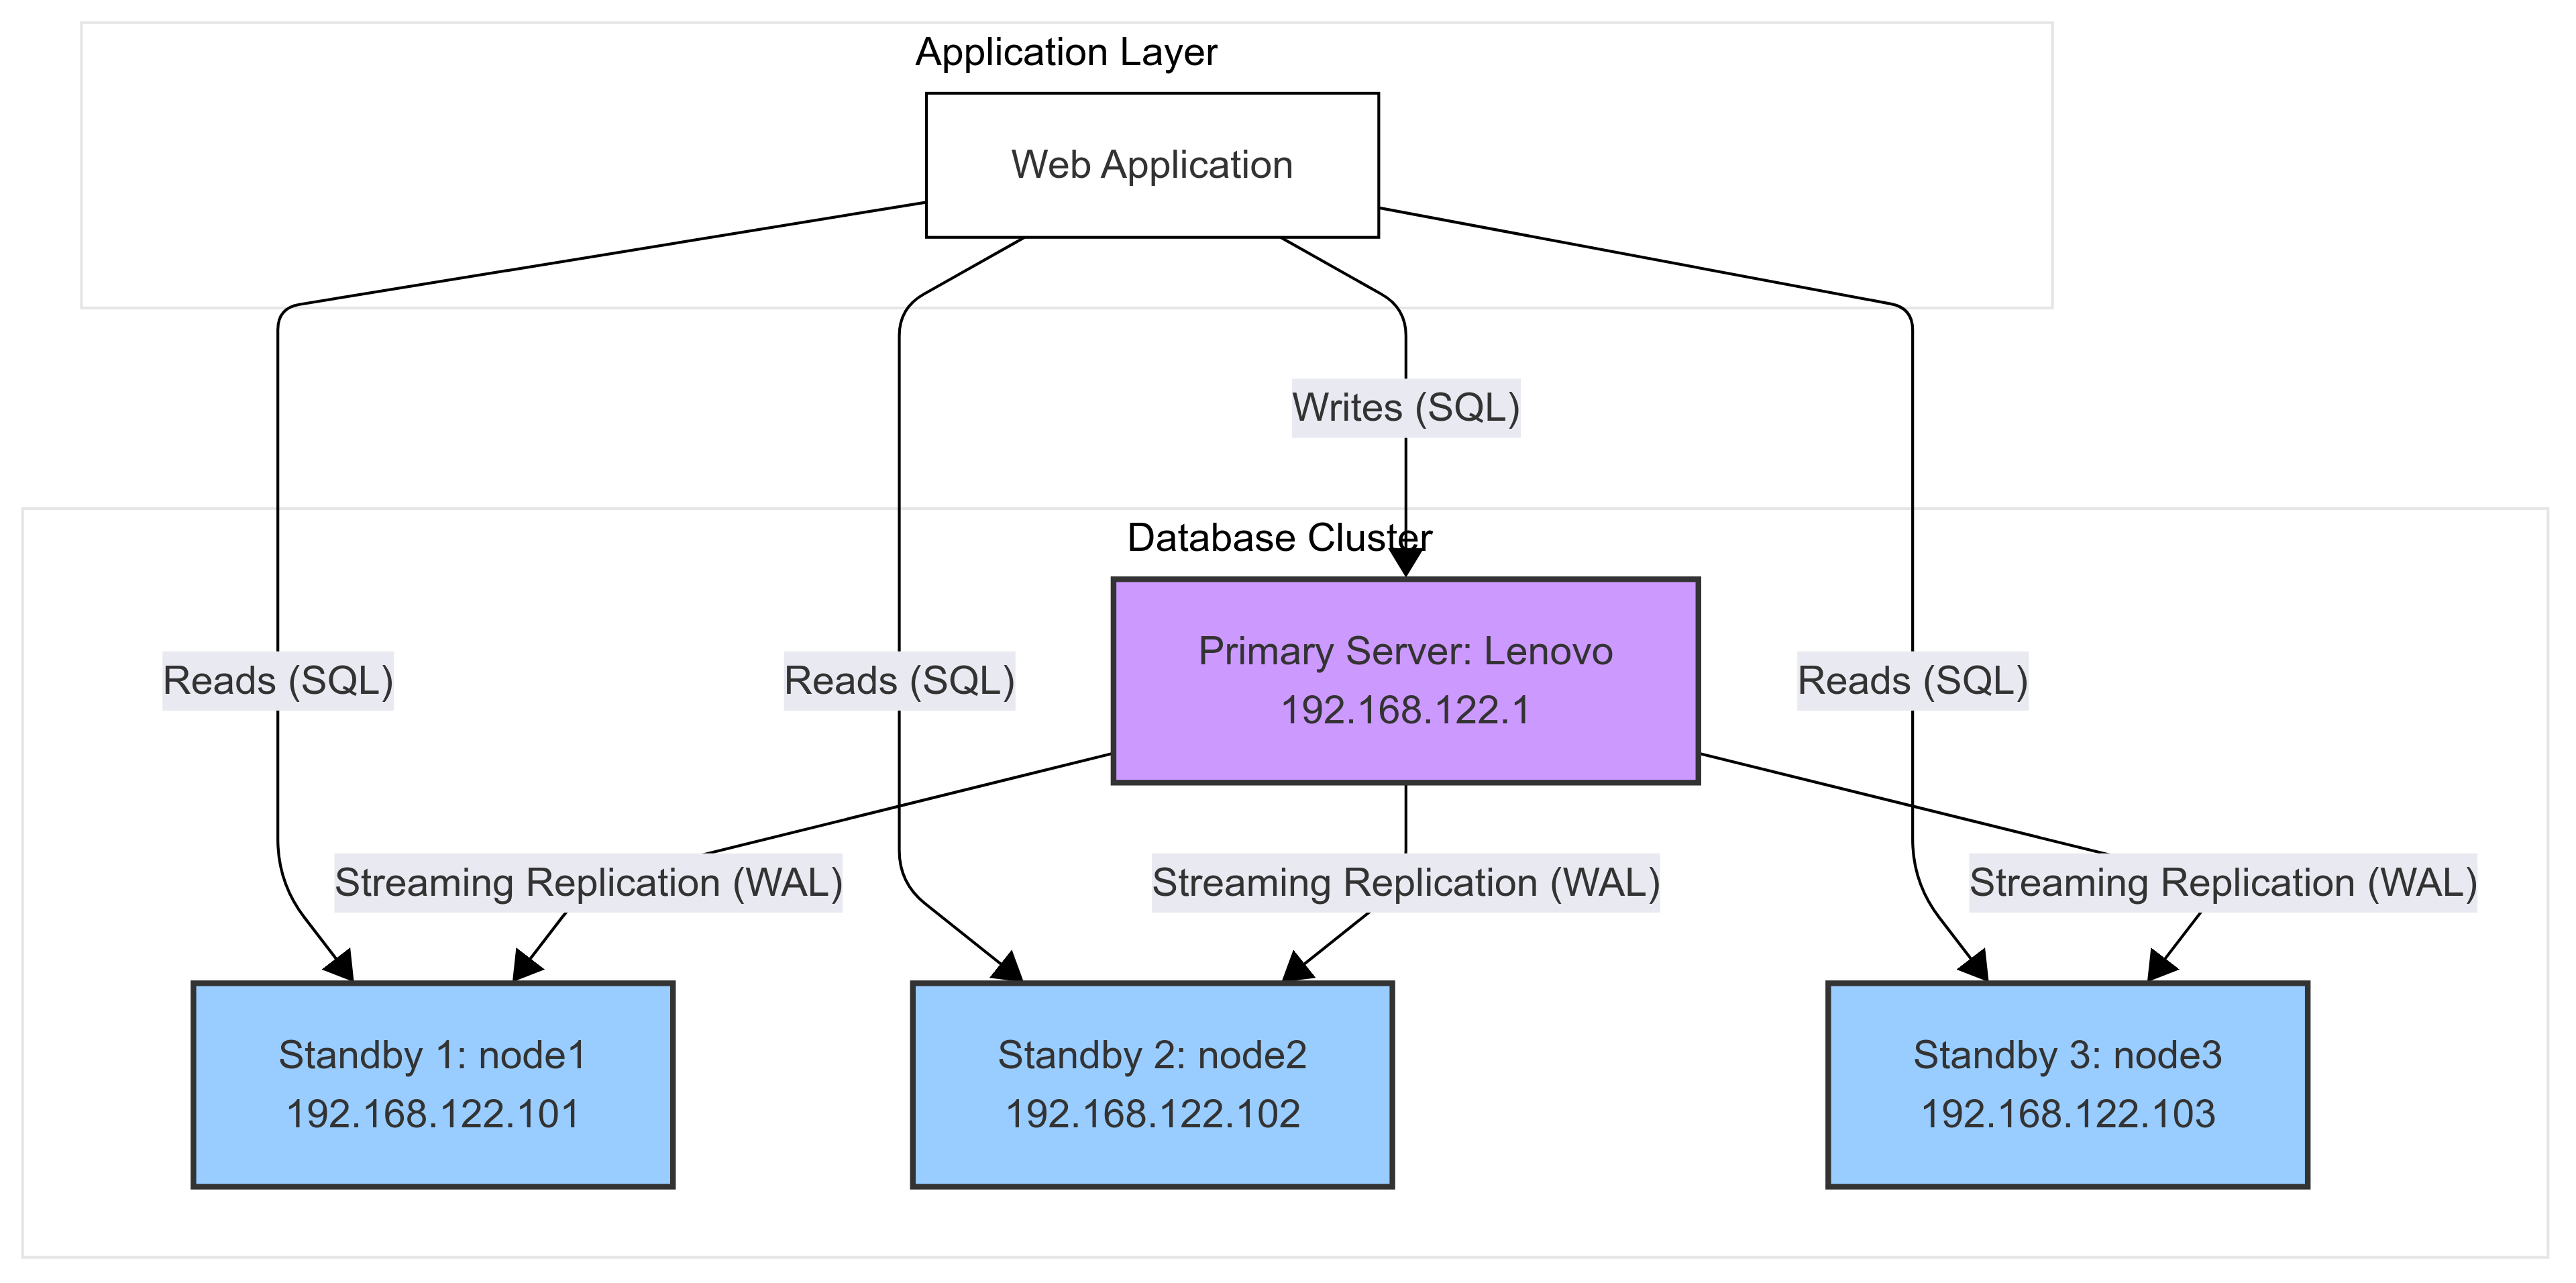
\includegraphics[width=0.9\columnwidth]{./images/architecture-diagram.png}
    \caption{The high-level architecture of the four-node replicated PostgreSQL cluster, showing the flow of write/read queries and the WAL replication stream.}
    \label{fig:architecture}
\end{figure}

\begin{table}[h!]
\centering
\caption{Node Configuration for the Distributed Cluster}
\label{tab:node_config}
\begin{tabular}{l l l l}
\toprule
\textbf{Role} & \textbf{Hostname} & \textbf{Operating System} & \textbf{Static IP Address} \\
\midrule
Primary   & Lenovo & EndeavourOS (Host) & 192.168.122.1 \\
Standby 1 & node1             & Ubuntu Server 24.04  & 192.168.122.101 \\
Standby 2 & node2             & Ubuntu Server 24.04  & 192.168.122.102 \\
Standby 3 & node3             & Ubuntu Server 24.04  & 192.168.122.103 \\
\bottomrule
\end{tabular}
\end{table}

\subsection{Standby Node Preparation}

To ensure consistency across all replicas and to streamline the setup process, I chose to create a master template rather than configuring each virtual machine from scratch.

I began by building this template, which is often referred to as a "golden image." This involved a minimal installation of Ubuntu Server 24.04 on a KVM virtual machine, followed by applying all system updates and installing PostgreSQL version 17 to match the primary server.

With the template finalized, I cloned it three times to create the node1, node2, and node3 VMs. Each clone, being an identical copy, required a unique identity on the network. For each VM, I performed the following configuration steps:

\begin{enumerate}

\item \textbf{Assigned a Unique Hostname:} I used the hostnamectl command to set a distinct name for each server (e.g., node1).

\item \textbf{Set a Static IP Address:} I edited the Netplan configuration file (/etc/netplan/) to assign the static IP corresponding to the node's role.

\item \textbf{Verified Connectivity:} I used the ping command from each standby to confirm it could reach the primary server and the other standby nodes.

\end{enumerate}

The final preparatory step was to stop the PostgreSQL service on each of these newly cloned standbys. This was a critical action, as their default data directories needed to be empty before being replaced by a binary copy of the primary server's data.

\subsection{Primary Server Configuration}

Before the standbys could connect, I had to configure the primary server (Lenovo) to accept incoming replication connections securely. This involved two main tasks.

First, I edited the primary's configuration files. In postgresql.conf, I set listen\_addresses to allow network connections and ensured wal\_level was set to replica. The replica setting is the minimum level that writes enough information to the Write-Ahead Log (WAL) to support streaming replication. Next, I had to configure the primary's security rules. A normal database connection is for accessing a specific database like 'pagila'. However, a replication connection is more powerful, as it needs access to the entire server's stream of data changes. To control this, I added a specific rule to the pg\_hba.conf file, which acts as PostgreSQL's firewall. This rule defines three conditions: the connection's purpose must be replication, it must be initiated by the replicator user, and it must come from the secure IP address range of my standby servers. This ensures that only my authorized standby servers can request the database's stream of changes.
Second, to make the replication link more robust, I implemented Replication Slots. This PostgreSQL feature provides a guarantee that the primary will not discard WAL files needed by a standby, even if that standby is disconnected for a long time. On the primary server, I created a unique, named slot for each of the three standby nodes.

\begin{lstlisting}[language=sql, caption={Creating a dedicated replication slot for each standby on the Primary.}, label={lst:create_slots}]
SELECT pg_create_physical_replication_slot('node1_slot');

SELECT pg_create_physical_replication_slot('node2_slot');

SELECT pg_create_physical_replication_slot('node3_slot');

\end{lstlisting}

After these changes, I restarted the primary PostgreSQL service to apply them. 

\subsection{Standby Replication Setup and Verification}

Once the primary server was ready with its replication slots, the next step was to set up each standby. This meant copying the primary's entire database and then telling the standby how to follow the primary's changes.

To do this, I used the \texttt{pg\_basebackup} tool. I ran the command from each standby server, pointing it at the primary. This copied all the data files and, thanks to the \texttt{-R} flag, it also automatically wrote the basic connection settings into a file named \texttt{postgresql.auto.conf} on the standby.
\begin{lstlisting}[language=bash, caption={Cloning the primary database to a standby.}]
sudo -u postgres pg_basebackup -h Lenovo -U replicator -D /var/lib/postgresql/17/main -P -R -Xs
\end{lstlisting}

The \texttt{pg\_basebackup} command sets up the basic connection, but it doesn't know about the specific replication slot I created for each server. To assign the unique slot, I used the \texttt{ALTER SYSTEM} command. This required a specific sequence: I had to start the standby's PostgreSQL service once to connect and run the command, and then restart it a second time for the new setting to be applied. For \texttt{node1}, the command I ran was:
\begin{lstlisting}[language=sql, caption={Assigning the unique slot using ALTER SYSTEM on standby node1.}, label={lst:alter_system}]
ALTER SYSTEM SET primary_slot_name = 'node1_slot';
\end{lstlisting}

I repeated these same steps for \texttt{node2} and \texttt{node3}, assigning them \texttt{node2\_slot} and \texttt{node3\_slot} respectively.

After restarting all the standbys for the final time, I checked the \texttt{pg\_stat\_replication} and \texttt{pg\_replication\_slots} views on the primary server to confirm everything was working. The queries showed all three standby nodes connected and actively streaming, which meant the cluster was fully operational.


\section{Analysis and Interpretation}
With the four-node cluster up and running, the next logical step was to put it to the test. I wanted to see if the architecture I built actually solved the two main problems I set out to address: handling a heavy read workload and surviving a server failure.

\subsection{Read Scalability Analysis}
The most immediate benefit of having three hot-standby servers is how it solves the "too popular" problem. I confirmed that I could connect directly to any of the standby nodes and run SELECT queries, while any INSERT or UPDATE commands were correctly rejected.

This means that in a real-world scenario, a load balancer could be used to direct all the Browse and searching traffic—which makes up most of a user's activity—to these three replicas. This strategy would free up the primary server almost entirely, leaving its resources dedicated to the less frequent but more critical tasks of processing new rentals or user sign-ups. The end result is a system that can handle a much larger volume of read traffic without slowing down, because the work is effectively shared across multiple machines.

\subsection{High Availability Analysis}
To test the "everything is broken" problem, I simulated a disaster by intentionally shutting down the primary server's database service. The result was exactly what I had hoped for. The standby servers didn't crash; they simply noted the lost connection in their logs and continued running.

I was still able to connect to a standby server and run read queries against the database, proving that the website wouldn't go completely offline in this scenario. Of course, any attempt to write new data failed, as the primary was the only server authorized to accept changes. The system had successfully entered a safe, read-only mode.

To restore full functionality, a manual failover would be required, where I would need to promote one of the standbys to become the new primary. The use of replication slots, which I implemented, is what makes this process reliable. Because each standby has a reserved slot, I have a guarantee that it can always reconnect and get back in sync after a downtime, making the recovery process predictable and safe from the common issue of a broken replication link.

\section{Conclusions and Recommendations}

\subsection{Conclusion}

This project set out to build a database system that could withstand the pressures of a popular web application, and I can confidently say it was a success. I successfully constructed a four-node PostgreSQL cluster, with one primary server replicating its data in real-time to three hot-standby servers. By implementing replication slots, I created a resilient link between the nodes, which guarantees that a standby can always recover its connection to the primary after a downtime.

My analysis showed that this architecture directly solves the two key problems of scalability and availability. The standby servers proved effective at handling read queries, which would allow a real application to distribute its workload and remain responsive under heavy user traffic. Furthermore, my simulation of a primary server failure demonstrated that the system maintains read-only service, successfully avoiding a complete shutdown.

Beyond the final result, this project provided invaluable hands-on experience with the practical challenges of setting up a distributed system, from network configuration and virtualization to advanced database administration.

\subsection{Recommendations}

While the cluster is fully functional as a proof-of-concept, several key steps would be needed to make it truly production-ready. Based on my analysis, I would recommend the following improvements:

\begin{itemize}
\item \textbf{Implement Automated Failover:} The current manual failover process, while effective, is slow and requires human intervention during a crisis. The next logical step would be to implement a tool like Patroni, an industry-standard cluster manager for PostgreSQL. It would monitor the primary's health and automatically promote a standby server in seconds if a failure is detected, dramatically improving recovery time.

\item \textbf{Establish Comprehensive Monitoring:} To properly manage a cluster, you need to be able to see its health in real-time. I would integrate a monitoring stack using Prometheus and Grafana. This would provide dashboards to track critical metrics like replication lag, transaction throughput, and server CPU usage, allowing for proactive maintenance before problems occur.

\end{itemize}
\appendices

\section{Configuration Snippets}

All materials related to this project, including the LaTeX source for this report, configuration file examples, and the detailed `README.md` guide, are publicly available in the following GitHub repository:

\url{https://github.com/finnzxje/INT14148}

\begin{thebibliography}{9}
\bibitem{postgres_replication}
The PostgreSQL Global Development Group, "Chapter 26. High Availability, Load Balancing, and Replication," \emph{PostgreSQL 17 Documentation}, 2024. [Online]. Available: \url{https://www.postgresql.org/docs/17/high-availability.html}
\bibitem{pagila}
"Pagila Sample Database," \emph{PostgreSQL Wiki}. [Online]. Available: \url{https://github.com/devrimgunduz/pagila}
\bibitem{ozsu_valduriez_2020}
M. T. Özsu and P. Valduriez, \emph{Principles of Distributed Database Systems}, 4th~ed.\hskip 1em plus 0.5em minus 0.4em\relax Cham, Switzerland: Springer, 2020.


\end{thebibliography}

%
%
%
%
%
%
%
%
%
%
\end{document}


